\section{Multiple distributions overlapped}
This input is similar to the mixed input from the last subsection.
For this distribution the values are not chosen uniform random from one of the base distributions, but instead a value from every distribution is chosen and added together.
Hence the name overlapped distribution.
For this input the step limit was increased to $100\cdot n \ln n$.
The comparison with the step limit $10\cdot n \ln(n)$ is contained in the last subsubsection which compares the best variants.

\begin{figure}[h]
      \caption{Distribution of an overlapped input with \textasciitilde$U(1,999)$, \textasciitilde$B(1000,0.1)$, \textasciitilde$Geo(0.01)$, powerlaw dist with $\beta=-1.25$}
      \centering
      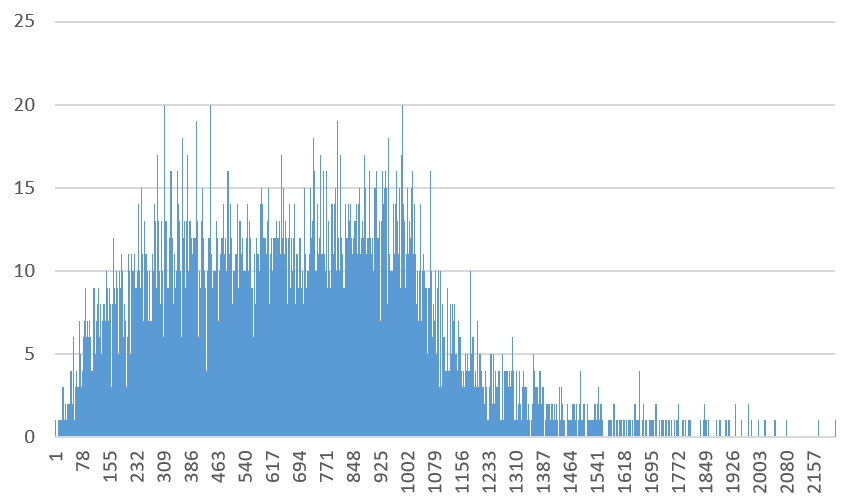
\includegraphics[width=0.7\textwidth]{figures/images/numberGenerator/overlapped.png}\label{fig:overlappedDistExample}
\end{figure}

Figure~\ref{fig:overlappedDistExample} looks completely different from figure~\ref{fig:mixedDistExample}.
No value is generated more than 20 times as opposed to the maximum amount of 350 for the mixed distribution.
In this figure no distribution is clearly visible.

The used distributions were \textasciitilde$U(1,49999)$, \textasciitilde$B(10000,0.1)$, \textasciitilde$Geo(0.001)$, powerlaw distribution with $\beta=-1.25$.
\subsection{RLS Comparison}


\makebox[\linewidth]{
\begin{tabular}{lp{3cm}p{6cm}p{6cm}}
\begin{tabular}[h]{cccccccc}
algo type&            \RLSN&     \RLSR&     \RLSR&     \RLSN&     \RLSR&     \RLSN&       RLS\\
algo param&             b=2&       s=3&       s=4&       b=3&       s=2&       b=4&         -\\
avg mut/change&       2.000&     1.996&     2.476&     3.000&     1.502&     4.000&     1.000\\
avg mut/step&         2.000&     2.000&     2.500&     3.000&     1.500&     4.000&     1.000\\
\hline
total avg count&     83,118&   104,748&   105,513&   112,223&   114,486&   121,927& 2,443,567\\
avg eval count&      83,118&   104,748&   105,513&   112,223&   114,486&   121,927&    45,834\\
max eval count&     778,110& 1,453,252&   898,974& 1,377,471&   915,268&   816,633&   485,275\\
min eval count&         197&       126&        45&       212&       271&       155&       128\\
\hline
fail ratio&           0.000&     0.000&     0.000&     0.000&     0.000&     0.000&     0.447\\
avg fail dif&             -&         -&         -&         -&         -&         -&         1\\
\end{tabular}
\end{tabular}
}


The results for this distribution are somewhat similar to the results of the binomial distribution.
The best and worst algorithms are the same.
Only the RLS almost fails to find an optimal solution for almost every input.
For the binomial distribution the $RLS-N_3$ also failed around 25\% or the inputs but here it does not.
It is even the second-best variant instead of being the second-worst.
Apart from that the ranking in between is also different.
The RLS-N variants perform the best followed by the RLS-R variants and lastly the RLS.
For the RLS-N the performance decreases with increasing $k$ but for the RLS-R this relation is inverted.
Another big difference is the number of steps needed to find a global optimum.
For the binomial input all algorithms except the RLS were really fast and only needed below 1000 iterations on average.
All algorithms need around 250 times the number of steps on average for the overlapped input.
This caused some of them to not be fast enough to solve the input always in time $10n\ln(n)$.
\subsection{(1+1) EA Comparison}


\makebox[\linewidth]{
\begin{tabular}{lp{3cm}p{6cm}p{6cm}}
\begin{tabular}[h]{ccccccccc}
algo type&          (1+1) EA&   (1+1) EA&   (1+1) EA&   (1+1) EA&      (1+1) EA&   (1+1) EA&   (1+1) EA&   (1+1) EA\\
algo param&           3/n&     4/n&     2/n&     5/n&       -&    10/n&    50/n&   100/n\\
avg mut/change&     3.101&   3.968&   2.343&   4.859&   1.698&   9.732&  49.544&  99.494\\
avg mut/step&       2.999&   4.003&   2.002&   4.999&   1.001&   9.998&  49.998&  99.997\\
\hline
total avg count&      646&     701&     706&     857&   1,123&   1,508&   8,175&  15,485\\
avg eval count&       646&     701&     706&     857&   1,123&   1,508&   8,175&  15,485\\
max eval count&     5,346&   5,692&   3,415&   5,572&   7,001&  12,112&  52,831& 145,269\\
min eval count&        23&       4&      30&       9&      23&      14&      27&      69\\
\hline
fails&                  0&       0&       0&       0&       0&       0&       0&       0\\
fail ratio&         0.000&   0.000&   0.000&   0.000&   0.000&   0.000&   0.000&   0.000\\
avg fail dif&           -&       -&       -&       -&       -&       -&       -&       -\\
\end{tabular}
\end{tabular}
}


The results for the (1+1) EA are similar but not the same.
Algorithms that had a good runtime on binomial inputs also have a good runtime in the overlapped runs, but the ranking is not the same.
For this input every the first and second place switched, the same for 3rd and 4th and also for 5th and 6th place.
This may be only caused by chance and the performance within a pair being really close but might also be caused by something else.
The (1+1) EA variants also needed about 200 times as long as for the binomial inputs.
All variants had at least 2 runs where they did not find an optimal solution.
These runs all had a remaining difference of one to the optimal value.
More time would probably be enough to reach an optimal solution in most cases.
\subsection{pmut Comparison}


\makebox[\linewidth]{
\scriptsize
\begin{tabular}{lp{3cm}p{6cm}p{6cm}}
\begin{tabular}[h]{m{2.5cm}m{0,40cm}m{0,40cm}m{0,40cm}m{0,40cm}m{0,40cm}m{0,40cm}m{0,40cm}m{0,40cm}m{0,40cm}m{0,40cm}m{0,40cm}m{0,40cm}m{0,40cm}m{0,40cm}m{0,40cm}m{0,40cm}m{0,40cm}m{0,40cm}}
\multicolumn{1}{c}{algo type}&\multicolumn{2}{c}{            pmut}&\multicolumn{2}{c}{     pmut}&\multicolumn{2}{c}{     pmut}&\multicolumn{2}{c}{     pmut}&\multicolumn{2}{c}{     pmut}&\multicolumn{2}{c}{     pmut}&\multicolumn{2}{c}{     pmut}&\multicolumn{2}{c}{     pmut}&\multicolumn{2}{c}{     pmut}\\
\multicolumn{1}{c}{algo param}&\multicolumn{2}{c}{           3.25}&\multicolumn{2}{c}{     3.00}&\multicolumn{2}{c}{     2.75}&\multicolumn{2}{c}{     2.50}&\multicolumn{2}{c}{     2.25}&\multicolumn{2}{c}{     2.00}&\multicolumn{2}{c}{     1.75}&\multicolumn{2}{c}{     1.50}&\multicolumn{2}{c}{     1.25}\\
\multicolumn{1}{c}{avg mut/change}&\multicolumn{2}{c}{      1.583}&\multicolumn{2}{c}{    1.737}&\multicolumn{2}{c}{    2.002}&\multicolumn{2}{c}{    2.423}&\multicolumn{2}{c}{    3.303}&\multicolumn{2}{c}{    5.830}&\multicolumn{2}{c}{   12.519}&\multicolumn{2}{c}{   30.910}&\multicolumn{2}{c}{   73.182}\\
\multicolumn{1}{c}{avg mut/step}&\multicolumn{2}{c}{        1.729}&\multicolumn{2}{c}{    1.934}&\multicolumn{2}{c}{    2.274}&\multicolumn{2}{c}{    2.895}&\multicolumn{2}{c}{    4.360}&\multicolumn{2}{c}{    8.452}&\multicolumn{2}{c}{   22.278}&\multicolumn{2}{c}{   70.532}&\multicolumn{2}{c}{  224.421}\\
\hline
\multicolumn{1}{c}{avg eval count}&\multicolumn{2}{c}{        540}&\multicolumn{2}{c}{      569}&\multicolumn{2}{c}{      594}&\multicolumn{2}{c}{      641}&\multicolumn{2}{c}{      712}&\multicolumn{2}{c}{      808}&\multicolumn{2}{c}{      967}&\multicolumn{2}{c}{    1,285}&\multicolumn{2}{c}{    2,081}\\
\multicolumn{1}{c}{max eval count}&\multicolumn{2}{c}{      3,110}&\multicolumn{2}{c}{    2,891}&\multicolumn{2}{c}{    3,504}&\multicolumn{2}{c}{    3,896}&\multicolumn{2}{c}{    5,152}&\multicolumn{2}{c}{    4,274}&\multicolumn{2}{c}{    5,610}&\multicolumn{2}{c}{    6,190}&\multicolumn{2}{c}{   14,984}\\
\multicolumn{1}{c}{min eval count}&\multicolumn{2}{c}{         22}&\multicolumn{2}{c}{        9}&\multicolumn{2}{c}{       36}&\multicolumn{2}{c}{       25}&\multicolumn{2}{c}{       28}&\multicolumn{2}{c}{       27}&\multicolumn{2}{c}{       27}&\multicolumn{2}{c}{       13}&\multicolumn{2}{c}{       33}\\
\hline
\multicolumn{1}{c}{fail ratio}&\multicolumn{2}{c}{          0.000}&\multicolumn{2}{c}{    0.000}&\multicolumn{2}{c}{    0.000}&\multicolumn{2}{c}{    0.000}&\multicolumn{2}{c}{    0.000}&\multicolumn{2}{c}{    0.000}&\multicolumn{2}{c}{    0.000}&\multicolumn{2}{c}{    0.000}&\multicolumn{2}{c}{    0.000}\\
\hline
\multicolumn{1}{c}{p-value}&&\multicolumn{2}{c}{0.0000}&\multicolumn{2}{c}{0.0000}&\multicolumn{2}{c}{0.0000}&\multicolumn{2}{c}{0.0000}&\multicolumn{2}{c}{0.0000}&\multicolumn{2}{c}{0.0000}&\multicolumn{2}{c}{0.0000}&\multicolumn{2}{c}{0.0000}\\
&&&&&&&&&&&&&&&&&&\end{tabular}
\end{tabular}
}


For $pmut$ the results are mostly the same as for the (1+1) EA.
The performance is about 250 times worse than for the binomial inputs, but the ranking is still pretty close.
Here the optimal parameter is around $\beta=-1.75$ instead of $\beta=-2.25$.
For $pmut$ the step limit was too small as well, but the difference to the optimal solution was only one on average.
\subsection{Comparison of the best variants}


\makebox[\linewidth]{
\begin{tabular}{lp{3cm}p{6cm}p{6cm}}
\begin{tabular}[h]{cccc}
algo type&            RLS&    pmut&      EA\\
algo param&             -&    3.25&       -\\
avg mut/change&     1.000&   1.287&   1.272\\
avg mut/step&       1.000&   1.729&   1.000\\
\hline
avg eval count&    91,171& 143,121& 231,082\\
max eval count&   153,143& 227,737& 446,942\\
min eval count&    65,783&  93,602& 165,818\\
\hline
fail ratio&         0.000&   0.000&   0.000\\
\end{tabular}
\end{tabular}
}


The results here are the same as for the binomial input. The $RLS-N_2$ performs better than the (1+1) EA and $pmut_\beta$ mutation for all values of $c/n$ and $\beta$ by a factor of 1.5 with a step limit of $10 \cdot n \ln(n)$. For the lower values of $n$ this does not hold to that extreme.

\begin{tabular}[h]{ccccccccc}
fails in 1000 runs&20&50&100&500&1000&5000&10000&50000\\\hline
RLS&984&773&411&1&0&0&0&0\\
\RLSR[2]&890&241&14&0&0&0&0&0\\
(1+1) EA (1$/n$)&711&75&5&0&0&0&0&0\\
(1+1) EA (2$/n$)&541&14&0&0&0&0&0&0\\
pmut (3.0)&566&63&4&0&0&0&0&0\\
pmut (3.25)&587&63&7&0&0&0&0&0\\
\end{tabular}


Here almost no algorithm manages to find an optimal solution in most cases as all algorithms fail for more than 70 \% of the inputs.
The RLS variants perform the worst again for the small input sizes.
Only for $n\ge500$ the $RLS-N_{2}$ is a good option due to the huge performance increase between $n=100$ and $n=500$.
Overlapped inputs stay hard to solve relatively long as only for $n\ge50,000$ all best variants of each algorithm find an optimal solution for every input.

\begin{tabular}[h]{ccccccccc}
avg&20&50&100&500&1000&5000&10000&50000\\\hline
RLS&32&79&153&579&950&1859&1922&1797\\
\RLSR[2]&391&2124&5005&4218&3530&2362&2160&2229\\
(1+1) EA (1$/n$)&22471&18343&12834&8342&6511&3815&3458&3371\\
(1+1) EA (2$/n$)&16360&9243&6452&4503&4020&3171&3141&3133\\
pmut (3.25)&23440&15929&9658&5644&4406&2434&2162&2172\\
pmut (3.0)&21901&14696&9186&5222&4150&2510&2208&2213\\
\end{tabular}


For $n\le1000$ the performance seems almost constant, but this is caused by the constant step limit of 100,000.
After $n=1000$ the value of $10 \cdot n \ln(n)$ was bigger than 100,000.

\begin{tabular}[h]{ccccccccc}
total avg&20&50&100&500&1000&5000&10000&50000\\\hline
RLS&99470&93459&74385&3474&447&389&421&555\\
\RLSR[2]&96305&63088&19364&815&589&565&595&699\\
(1+1) EA (1$/n$)&89444&52886&21141&1410&869&850&875&1046\\
(1+1) EA (2$/n$)&79603&37214&14107&1302&992&942&957&1055\\
pmut (3.25)&84226&48403&18280&930&542&526&546&642\\
pmut (3.0)&82474&46286&17825&917&576&548&573&668\\
\end{tabular}



No algorithm is very successful for the small values of $n$.
Choosing the (1+1) EA for $n<500$ should result in the best runtime in most of the cases.
Only the $RLS-N_4$ is faster for $50\le n \le 100$.
For bigger input sizes the $RLS-N_2$ is clearly the best option.
